\documentclass[12pt]{article}
\usepackage[utf8]{inputenc}
\usepackage{float}
\usepackage{amsmath}
\usepackage{tikz} % for Hasse diagram
\usepackage[hmargin=3cm,vmargin=6.0cm]{geometry}
%\topmargin=0cm
\topmargin=-2cm
\addtolength{\textheight}{6.5cm}
\addtolength{\textwidth}{2.0cm}
%\setlength{\leftmargin}{-5cm}
\setlength{\oddsidemargin}{0.0cm}
\setlength{\evensidemargin}{0.0cm}

\begin{document}
	
\section*{Student Information } 
%Write your full name and id number between the colon and newline
%Put one empty space character after colon and before newline
Full Name : Ugur Duzel \\
Id Number : 2171569  \\

% Write your answers below the section tags
\section*{Answer 1}
Let $a_n$ be the number of ternary string that contain three consecutive 0's, 1's or 2's. We will find a recurrence relation for $a_n$ by exploiting the symmetry rule among 0, 1, 2. $\frac{a_n}{3}$ such strings must start with each of the three options - 0, 1, 2. We should specify a string of length n satisfying the condition of consisting three consecutive 0's, 1's or 2's. \\
We can choose the first element in any of the three ways. We can follow this by string that starts with a different element, there are $\frac{2a_{n-1}}{3}$ such strings. Alternatively, we can follow the first symbol with itself. At this point, we have two elements that are the same (namely ...00, ...11, ...22). \\
We now have two paths like we had at the beginning. We can follow the first and the second element with a string that starts with a different element, there are $\frac{2a_{n-2}}{3}$ such strings. Alternatively again, we can follow the first and the second elements with themselves (namely ...000, ...111, ...222). In this case we already have a existing three consecutive symbols so whatever the rest of $n-3$ length of the string is, the condition is already satisfied. There are $3^{n-3}$ such strings exist. \\
We have this method working for all three ways so,
$$a_n=3(\frac{2a_{n-1}}{3}+\frac{2a_{n-2}}{3}+3^{n-3})$$
$$a_n=2a_{n-1}+2a_{n-2}+3^{n-2}$$


\section*{Answer 2}
\subsubsection*{a)}
There are three ways to do it. \\
\begin{figure}[H]
\centering
\begin{tikzpicture}
%%   kw   (name)   (x, y)   {text} 
    \draw (0,0) -- (0,1);
    \draw (0,0) -- (2,0);
    \draw (0,1) -- (0,2);
    \draw (0,1) -- (2,1);
    \draw (0,2) -- (2,2);
    \draw (2,2) -- (3, 2);
    \draw (2,0) -- (3,0);
    \draw (2,0) -- (2,1);    
    \draw (2,1) -- (2,2);
    \draw (3,0) -- (3,2);
\end{tikzpicture} \caption{Call it $T_1$}
\end{figure}
\begin{figure}[H]
\centering
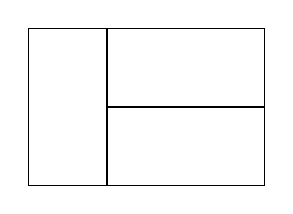
\begin{tikzpicture}
%%   kw   (name)   (x, y)   {text}
    \draw (0,0) -- (0, 1);
    \draw (0,0) -- (2, 0);
    \draw (0, 1) -- (0, 2);
    \draw (0, 1) -- (2, 1);
    \draw (0, 2) -- (2,2);
    \draw (0, 2) -- (-1, 2);
    \draw (0,0) -- (-1,0);
    \draw (2, 0) -- (2, 1);    
    \draw (2, 1) -- (2, 2);
    \draw (-1,0) -- (-1, 2);
\end{tikzpicture} \caption{Call it $T_2$}
\end{figure}
\begin{figure}[H]
\centering
\begin{tikzpicture}
%%   kw   (name)   (x, y)   {text}
    \draw (0,0) -- (1, 0);
    \draw (1, 0) -- (2, 0);
    \draw (0, 2) -- (1, 2);
    \draw (1, 2) -- (2, 2);
    \draw (0,0) -- (0, 2);
    \draw (1, 0) -- (1, 2);
    \draw (2, 0) -- (2, 2);
    \draw (2, 0) -- (3, 0);    
    \draw (2, 2) -- (3, 2);
    \draw (3, 0) -- (3, 2);       
\end{tikzpicture} \caption{Call it $T_3$}
\end{figure}
\subsubsection*{b)}
There is no possible way to totally cover the 3xn board with 3x2 tiles if n is an odd number. That's why at the end I will give the answer in a piecewise form. \\
If we want to construct a length n board, we should take n-2 already tiled board and append it a new tile. The same way if we want to construct a length n-2 board, we should take n-4 already tiled board and append it a new tile. This goes until my initial conditions. This is where a recurrence relation occurs to me. \\
The question asks for length n board so we should take n-2 already tiled board, the combination of the tiles doesn't matter. We don't need to think about the n-2 part, our recursive algorithm will think for us ("AST", best regards to Gokturk Hoca). I only need to specify the initial condition which is $a_2=2$\\
Now it time for the tricky part of this question. For the tile we append at the end of the already tiled board of length n-2, we have 3 alternatives named $T_1,T_2,T_3$ from part-a, this gives us $3a_{n-2}$ part. Although, there is only one possibility we count more than one time. If n-2 part is all $T_3$ and we append $T_1$ and $T_2$ they will be the same board and we will be counting them twice, this gives us the $-1$ part. The solution is going to be,
$$
a_n = \left\{
        \begin{array}{ll}
            0 & \quad n \equiv 1\mod 2 \\
            3a_{n-2}-1 & \quad n \equiv 0\mod 2 \\
        \end{array}
    \right.
$$
$$4 \leq n$$
$$a_2=2$$
\vspace{2cm}
\subsubsection*{c)}
\begin{equation} 
\begin{split}
a_n & = 3a_n - 1, (4 \leq n) \\
a_{2k} & = 3a_{2k-2}-1, (2 \leq k,\ k \in \{2,3,4,...\}) \\ 
a_{2k+2} & = 3a_{2k}-1, (2 \leq k,\ k \in \{2,3,4,...\}) \\ 
G(x) & =\sum_{k=0}^{\infty}a_{2k+2}x^k = a_2x^0+a_4x^1+a_6x^2+...\\
xG(x) & =\sum_{k=0}^{\infty}a_{2k+2}x^{k+1}=\sum_{k=1}^{\infty}a_{2k}x^k \\ 
G(x)-3xG(x) 
& = \sum_{k=0}^{\infty}a_{2k+2}x^k-\sum_{k=1}^{\infty}3a_{2k}x^k \\
& = a_2x^0 + \sum_{k=1}^{\infty}(a_{2k+2}-3a_{2k})x^k \\
& = 2 - (x+x^2+x^3+...) \\
& = 2 - (\frac{1}{1-x}-1) \\
& = 3 - \frac{1}{1-x} \\
& = \frac{2-3x}{1-x} \\ \\
G(x)(1-3x) & =\frac{2-3x}{1-x}\\
G(x) & =\frac{2-3x}{(1-x)(1-3x)}\\
& = \frac{3}{2}.\frac{1}{1-3x}+\frac{1}{2}.\frac{1}{1-x} \\
& = \frac{3}{2}\sum_{k=0}^{\infty}3^kx^k+\frac{1}{2}\sum_{k=0}^{\infty}x^k \\ \\
G(x) & =  \sum_{k=0}^{\infty}\frac{(1+3^{k+1})}{2}x^k  \\
G(x) & =\sum_{k=0}^{\infty}a_{2k+2}x^k =  \sum_{k=0}^{\infty}\frac{(1+3^{k+1})}{2}x^k \\
a_{2k+2} & = \frac{(1+3^{k+1})}{2} \\
a_{2k} & = \frac{(1+3^k)}{2} \\
\end{split}
\end{equation}
\section*{Answer 3}
\subsubsection*{a)}
The relation has to satisfy all three properties - reflexive, anti-symmetry, transitive - to be a partial ordering. Let's say we have A, B as our sets. \\
- $A\subseteq A$ relation holds for every set since $A=A$. This means that the relation is reflexive on any set of sets.\\
- $A\subseteq B$ relation is known to exist then there shouldn't be the relation $B\subseteq A$ in order to be anti-symmetric. If both of these relations exist then it means $A=B$. This is not true since $A$ and $B$ must be different. So if $A\subseteq B$ exists, $B\subseteq A$ cannot exist. This means that the relation is anti-symmetric on any set of sets. \\
- $A\subseteq B$ and $B\subseteq C$ relations are known to exist, then we can say $A\subseteq B\subseteq C$ is true and clearly deduce that $A\subseteq C$. This means that the relation is transitive on any set of sets. 

\subsubsection*{b)}
The relation has to satisfy all three properties - reflexive, anti-symmetry, transitive - to be a partial ordering. Showing one non-satisfactory is enough to say this is not partial ordering. \\
Reflexive property satisfies all the integers expect 0. Since 0 is an integer reflexive property must satisfy for 0 as well. However, $0|0$ is undefined (undetermined). So this relation does not satisfy reflexivity on $Z$ due to the integer 0. That's why the relation is not a partial ordering of the set of integers.

\subsubsection*{c)}
The relation has to satisfy all three properties - reflexive, anti-symmetry, transitive - to be a partial ordering. Let's say $a, b, c \in Z$, \\ 
- $a\ R\ a$ is true since $a=a^r$ ($r \in Z^+$) when $r=1$. So the relation is reflexive on $Z$.\\
- $a\ R\ b$ is known to exist then we can say that $a=b^{r_1}$ ($r_1 \in Z^+$). In this situation, $b\ R\ a$ shouldn't exist so that the relation can be anti-symmetric. Moreover, $b\ R\ a$ cannot exist. If it existed, then we could say $b=a^{r_2}$ ($r_2 \in Z^+$) and looking at both of the equalities $r_1r_2=1$. Since we know $r_1$ is a positive integer, $r_2$ cannot be a positive integer. This contradicts with the relation, $r_2$ should have been a positive integer as well. So $b\ R\ a$ doesn't exist and the relation satisfies anti-symmetry on $Z$. \\
- $a\ R\ b$ and $b\ R\ c$ known to exist then we can say the following $a=b^{r_1}$, $b=c^{r_2}$ ($r_1,r_2 \in Z^+$). From this point we can deduce that $a=c^{r_1r_2}$. Since $r_1,r_2 \in Z^+$, we can introduce $r_3=r_1r_2$ and $r_3 \in Z^+$. Now we can say that $a=c^{r_3}$ and $a\ R\ c$. This means that the relation is transitive on $Z$. \\
In conclusion, the relation is partial ordering of $Z$.
\section*{Answer 4}
\subsubsection*{a)}
$P_1=\{\ 1,\ 1,\ 1,\ 1,\ 1\ \}$ \\
$P_2=\{\ 1,\ 1,\ 1,\ 2\ \}$ \\
$P_3=\{\ 1,\ 1,\ 3\ \}$ \\
$P_4=\{\ 2,\ 2,\ 1\ \}$ \\
$P_5=\{\ 1,\ 4\ \}$ \\
$P_6=\{\ 2,\ 3\ \}$ \\
$P_7=\{\ 5\ \}$ \\
\subsubsection*{b)}
%Hasse diagram example
\begin{figure}[H]
\centering
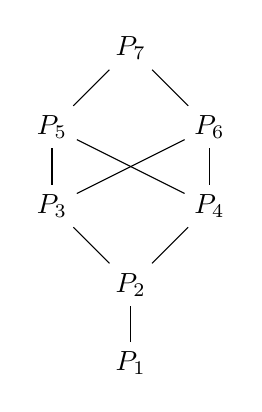
\begin{tikzpicture}
%%   kw   (name)   (x, y)   {text}
    \node (p7) at (2, 4)    {$P_7$};
    \node (p6) at (3, 3)     {$P_6$};
    \node (p5) at (3, 2)     {$P_4$};
    \node (p4) at (1, 3)     {$P_5$};
    \node (p3) at (1, 2)     {$P_3$};
    \node (p2) at (2, 1)     {$P_2$};
    \node (p1) at (2, 0)     {$P_1$};

    \draw (p1) -- (p2);
    \draw (p2) -- (p3);
    \draw (p2) -- (p5);
    \draw (p5) -- (p4);
    \draw (p5) -- (p6);
    \draw (p3) -- (p4);
    \draw (p3) -- (p6);
    \draw (p4) -- (p7);
    \draw (p6) -- (p7);
\end{tikzpicture} \caption{Diagram of $\{\ P_1,\ P_2,\ P_3,\ P_4,\ P_5,\ P_6,\ P_7\ \}$ ordered by  the given precedence relation}
\end{figure}

\end{document}